\documentclass[11pt,a4paper]{article}
\usepackage[margin=1in]{geometry}
\usepackage[T1]{fontenc}
\usepackage[utf8]{inputenc}
\usepackage{lmodern}
\usepackage{hyperref}
\usepackage{enumitem}
\usepackage{xurl}
\usepackage{tikz}
\usepackage{float}
\usetikzlibrary{arrows.meta, positioning, shapes.geometric}
\hypersetup{colorlinks=true,linkcolor=blue,urlcolor=blue}
\newcommand{\codepath}[1]{\path{#1}}
\tikzset{box/.style={rectangle,draw,rounded corners,align=center,inner sep=3pt,minimum width=36mm},line/.style={-Latex}}

\title{Phase-2 QEMU: Deliverable 2 (Adapter)}
\author{Senior Systems Architecture}
\date{\today}

\begin{document}
\maketitle

\section{Technical Description}
The QEMU adapter converts platform-native execution output into Phase-1 ingest contract intervals, preserving simulator independence of SIT computation.

\section{Implementation Fulfillment}
Implemented in \codepath{Phase-2/adapters/qemu_adapter.py}, invoked by \codepath{Phase-2/riscvbench.py} via \texttt{--target qemu}.
Adapter outputs:
\begin{itemize}[leftmargin=*]
  \item \codepath{inputs/state\_intervals.csv}
  \item \codepath{inputs/residency\_intervals.csv}
\end{itemize}

\section{Design \& Architecture}
The adapter is intentionally policy-thin: parsing + normalization + validation only. Windowing, SIT formula, and summary semantics remain in \codepath{Phase-2/sit_engine_phase1.py}.

\subsection*{Function Flowchart}
\begin{figure}[H]
\centering
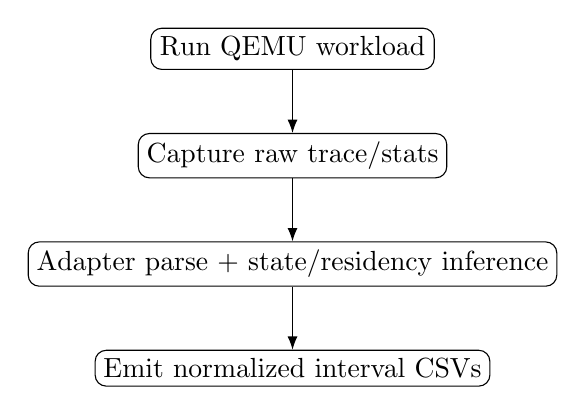
\begin{tikzpicture}[node distance=8mm and 12mm]
\node[box] (a) {Run QEMU workload};
\node[box, below=of a] (b) {Capture raw trace/stats};
\node[box, below=of b] (c) {Adapter parse + state/residency inference};
\node[box, below=of c] (d) {Emit normalized interval CSVs};
\draw[line] (a) -- (b);
\draw[line] (b) -- (c);
\draw[line] (c) -- (d);
\end{tikzpicture}
\caption{QEMU Adapter Flow}
\end{figure}

\end{document}
